\documentclass{beamer}
\usepackage{pgfpages}
%\setbeameroption{show notes on second screen=left} %enable for notes
\usepackage{graphicx}
\usepackage{xcolor}
\usepackage{listings}
%\usepackage{transparent}
\usepackage{hyperref}
\lstset{language=python,frame=single}
\usepackage{verbatim}
%\usepackage{apacite}
\usepackage[longnamesfirst]{natbib}
\usepackage{subcaption}
\usepackage{amsmath}
\usepackage{relsize}
\usepackage{appendixnumberbeamer}
\usepackage{xparse}
\usepackage{multimedia}
\usepackage{xcolor}
\usepackage[normalem]{ulem}
\usepackage{tikz}
\usetikzlibrary{matrix,backgrounds}
\usetikzlibrary{positioning}
\usetikzlibrary{shapes,arrows}
\usetikzlibrary{positioning}

\tikzset{onslide/.code args={<#1>#2}{%
  \only<#1>{\pgfkeysalso{#2}} 
}}

\tikzstyle{block} = [rectangle, draw, fill=red!20!blue!10, 
    text width=5em, text centered, rounded corners, minimum height=4em]
\tikzstyle{netnode} = [circle, draw, very thick, inner sep=0pt, minimum size=0.5cm] 
    
\tikzstyle{line} = [draw, line width=1.5pt, -latex']

\pgfdeclarelayer{background}
\pgfsetlayers{background,main}

\pgfdeclarelayer{myback}
\pgfsetlayers{myback,background,main}

\usetheme[numbering=fraction]{metropolis}

\newcommand\blfootnote[1]{%
  \begingroup
  \renewcommand\thefootnote{}\footnote{#1}%
  \addtocounter{footnote}{-1}%
  \endgroup
}
\renewcommand*\footnoterule{}
%%\AtBeginSection[]
%%{
%%  \begin{frame}
%%    \frametitle{Table of Contents}
%%    \tableofcontents[currentsection]
%%  \end{frame}
%%}

\begin{document}

\title{Toward a theory of transfer}
\author{Andrew Lampinen}
\date{Lightning Talk, Oct. 4th 2017}
\frame{\titlepage}

\begin{frame}{Transfer}
\begin{figure}
\centering
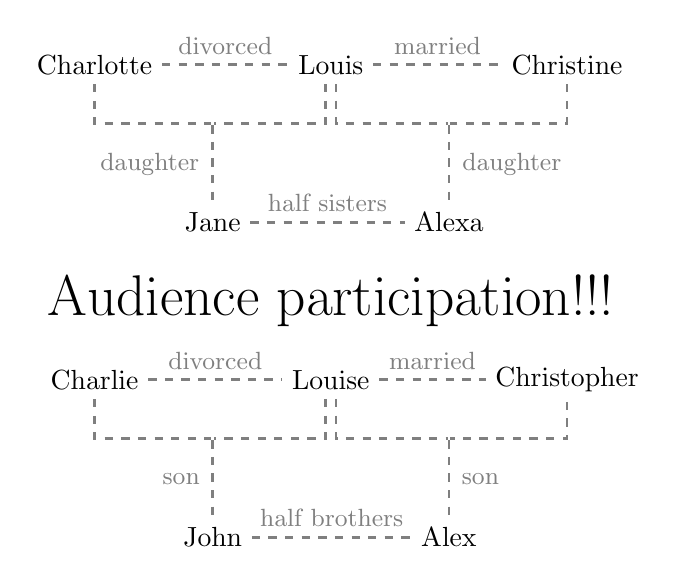
\begin{tikzpicture}[auto]
\only<1>{
\node at (0, -3) {\huge Audience participation!!!};
}
\uncover<2->{
\node at (0, 0) (Louis) {Louis};  
\node at (-3, 0) (p11) {Charlotte};
\path [draw, dashed, opacity=0.5, line width=1.0pt] (p11) -- node {\small divorced} (Louis);

\node at (-1.5, -0.75) [inner sep=0, outer sep=0] (m11) {};
\node at (-1.5, -2) (Jane) {Jane};
\path [draw, dashed, opacity=0.5, line width=1.0pt] (p11) |- (m11);
\path [draw, dashed, opacity=0.5, line width=1.0pt] ([xshift=-0.2cm]Louis) |- (m11);
\path [draw, dashed, opacity=0.5, line width=1.0pt] (m11) -- node [anchor=center, xshift=-0.8cm] {\small daughter} (Jane);

\node at (3, 0) (p12) {Christine};
\path [draw, dashed, opacity=0.5, line width=1.0pt] (Louis) -- node {\small married} (p12);

\node at (1.5, -0.75) [inner sep=0, outer sep=0] (m12) {};
\node at (1.5, -2) (Alexa) {Alexa};
\path [draw, dashed, opacity=0.5, line width=1.0pt] (p12) |- (m12);
\path [draw, dashed, opacity=0.5, line width=1.0pt] ([xshift=0.2cm]Louis) |- (m12);
\path [draw, dashed, opacity=0.5, line width=1.0pt] (m12) -- node [anchor=center, xshift=0.8cm] {\small daughter} (Alexa);
\path [draw, dashed, opacity=0.5, line width=1.0pt] (Jane) -- node {\small half sisters} (Alexa);
}
\begin{scope}[shift={(0, -4)}]
\uncover<3->{
\node at (0, 0) (Louise) {Louise};  
\node at (-3, 0) (p11) {Charlie};
\path [draw, dashed, opacity=0.5, line width=1.0pt] (p11) -- node {\small divorced} (Louise);
\node at (3, 0) (p12) {Christopher};
\path [draw, dashed, opacity=0.5, line width=1.0pt] (Louise) -- node {\small married} (p12);

\node at (-1.5, -0.75) [inner sep=0, outer sep=0] (m11) {};
\node at (-1.5, -2) (John) {John};
\path [draw, dashed, opacity=0.5, line width=1.0pt] (p11) |- (m11);
\path [draw, dashed, opacity=0.5, line width=1.0pt] ([xshift=-0.2cm]Louise) |- (m11);
\path [draw, dashed, opacity=0.5, line width=1.0pt] (m11) -- node [anchor=center, xshift=-0.4cm] {\small son} (John);
}
\uncover<4->{
\node at (1.5, -0.75) [inner sep=0, outer sep=0] (m12) {};
\node at (1.5, -2) (Alex) {Alex};
\path [draw, dashed, opacity=0.5, line width=1.0pt] (p12) |- (m12);
\path [draw, dashed, opacity=0.5, line width=1.0pt] ([xshift=0.2cm]Louise) |- (m12);
\path [draw, dashed, opacity=0.5, line width=1.0pt] (m12) -- node [anchor=center, xshift=0.4cm] {\small son} (Alex);
\path [draw, dashed, opacity=0.5, line width=1.0pt] (John) -- node {\small half brothers} (Alex);
}
\end{scope}
\end{tikzpicture}
\note{I'm gonna tell you about a family... Louis is divorced from Barbara but they have a daughter named Jane, and now Louis is married to Katie, and they have a daughter named Alexa}
\end{figure}

\blfootnote{\uncover<2->{\citep*{Hinton1986}}}
\end{frame}

\begin{frame}{The human condition}
\note{We've suggested that task analogies are much broader than this and may help explain why humans are able to learn so fast.}
\begin{figure}
\centering
\uncover<2->{%
\begin{subfigure}{0.5\textwidth}
\includegraphics[width=\textwidth]{figures/chess_cropped.jpg}
\end{subfigure}}%
\uncover<3->{%
\begin{subfigure}{0.5\textwidth}
\includegraphics[width=\textwidth]{figures/go.jpg}
\end{subfigure}}\\%
\uncover<4->{%
\begin{subfigure}{0.5\textwidth}
\includegraphics[width=\textwidth]{figures/math.jpg}
\end{subfigure}}%
\uncover<5->{%
\begin{subfigure}{0.5\textwidth}
\includegraphics[width=\textwidth]{figures/piano.jpg}
\end{subfigure}}%
\end{figure}
%\blfootnote{\citep*{Hansen2017}}
\nocite{Hansen2017, Lampinen2017}
\end{frame}

\begin{frame}[fragile]{Neural nets transfer too!}
\begin{figure}
\centering
\begin{tikzpicture}[remember picture, overlay, every node/.style={inner sep=0,outer sep=0}]
\node [anchor=center, outer sep=0, inner sep=0] at (current page.center) (brain) {\includegraphics[width=0.25\textwidth]{figures/google_brain.png}}; 
\node<2-> [anchor=center, below left = 1cm and 0.25cm of brain] (input1) {``Ceci n'est pas une pipe.''};
\node<2-> [anchor=center, above left = 1cm and 0.25cm of brain] (output1) {``This is not a pipe.''};

\node<3-> [anchor=center, below right = 0.45cm and 0.25cm of brain] (input2) {\includegraphics[width=0.25\textwidth]{figures/un_pipe.jpg}};
\node<3-> [anchor=center, above right = 1cm and 0.25cm of brain] (output2) {``This is a pipe.''};

\begin{pgfonlayer}{background}
\path<2-> [line] (input1.east) to [out=45, in=-45] (output1.east); 
\path<3-> [line] (input2.west) to [out=135, in=-135] (output2.west); 
\end{pgfonlayer}
\end{tikzpicture}
\end{figure}

%\blfootnote{\citep*{Luong2016}}
\nocite{Luong2016}
\end{frame}

\begin{frame}[standout]
We suggest that these are similar processes. \\
Can we develop a theory?
\end{frame}


%\section{Can we make a theory?}

\begin{frame}{Isomorphic tasks for neural networks}
\begin{figure}
\centering
\begin{tikzpicture}[auto]
\begin{scope}[shift={(-1.5, 0)}]
\node [text width=3cm, text centered, anchor=north] at (0,-0.33) (input1) {%
\only<1-4,10-13>{``Who are Alexa's parents?''}
};

\node [netnode, onslide={<2-4,11-13,15-17>{fill=red!20}}] at (-1,1) (h111) {};
\node [netnode, onslide={<2-4,11-13,15-17>{fill=red!90}}] at (0,1) (h112) {};
\node [netnode, onslide={<2-4,11-13,15-17>{fill=blue!60}}] at (1,1) (h113) {};

\path [draw, very thick] (input1.north) to (h111);
\path [draw, very thick] (input1.north) to (h112);
\path [draw, very thick] (input1.north) to (h113);

\node [netnode, onslide={<3-4,12-13,16-17>{fill=blue!20}}] at (-1,3) (h121) {};
\node [netnode, onslide={<3-4,12-13,16-17>{fill=red!40}}] at (0,3) (h122) {};
\node [netnode, onslide={<3-4,12-13,16-17>{fill=blue!40}}] at (1,3) (h123) {};

\path [draw, very thick] (h111) to (h121);
\path [draw, very thick] (h111) to (h122);
\path [draw, very thick] (h111) to (h123);
\path [draw, very thick] (h112) to (h121);
\path [draw, very thick] (h112) to (h122);
\path [draw, very thick] (h112) to (h123);
\path [draw, very thick] (h113) to (h121);
\path [draw, very thick] (h113) to (h122);
\path [draw, very thick] (h113) to (h123);

\node [anchor=south, align=center] at (0,4.33) (output1) {%
\only<4,13>{``Louis and\\ Christine''}
};

\path [draw, very thick] (h121) to (output1.south);
\path [draw, very thick] (h122) to (output1.south);
\path [draw, very thick] (h123) to (output1.south);
\end{scope}

\begin{scope}[shift={(1.5, 0)}]
\node [text width=3cm, text centered, anchor=north] at (0,-0.33) (input2) {%
\only<5-8,14-17>{``Who are Alex's parents?''}
};

\node [netnode, onslide={<6-8,11-13,15-17>{fill=red!40}}] at (-1,1) (h211) {};
\node [netnode, onslide={<6-8,11-13,15-17>{fill=blue!10}}] at (0,1) (h212) {};
\node [netnode, onslide={<6-8,11-13,15-17>{fill=blue!80}}] at (1,1) (h213) {};

\path [draw, very thick] (input2.north) to (h211);
\path [draw, very thick] (input2.north) to (h212);
\path [draw, very thick] (input2.north) to (h213);

\node [netnode, onslide={<7-8,12-13,16-17>{fill=red!60}}] at (-1,3) (h221) {};
\node [netnode, onslide={<7-8,12-13,16-17>{fill=red!30}}] at (0,3) (h222) {};
\node [netnode, onslide={<7-8,12-13,16-17>{fill=red!80}}] at (1,3) (h223) {};

\path [draw, very thick] (h211) to (h221);
\path [draw, very thick] (h211) to (h222);
\path [draw, very thick] (h211) to (h223);
\path [draw, very thick] (h212) to (h221);
\path [draw, very thick] (h212) to (h222);
\path [draw, very thick] (h212) to (h223);
\path [draw, very thick] (h213) to (h221);
\path [draw, very thick] (h213) to (h222);
\path [draw, very thick] (h213) to (h223);

\node [anchor=south, yshift=-0.07cm, align=center] at (0,4.33) (output2) {%
\only<8,17>{``Louise and\\ Christopher''}
};

\path [draw, very thick] (h221) to ([yshift=0.05cm]output2.south);
\path [draw, very thick] (h222) to ([yshift=0.05cm]output2.south);
\path [draw, very thick] (h223) to ([yshift=0.05cm]output2.south);
\end{scope}

\uncover<9->{
\path [draw, very thick] (input1.north) to (h211);
\path [draw, very thick] (input1.north) to (h212);
\path [draw, very thick] (input1.north) to (h213);
\path [draw, very thick] (input2.north) to (h111);
\path [draw, very thick] (input2.north) to (h112);
\path [draw, very thick] (input2.north) to (h113);
\path [draw, very thick] (h111) to (h221);
\path [draw, very thick] (h111) to (h222);
\path [draw, very thick] (h111) to (h223);
\path [draw, very thick] (h112) to (h221);
\path [draw, very thick] (h112) to (h222);
\path [draw, very thick] (h112) to (h223);
\path [draw, very thick] (h113) to (h221);
\path [draw, very thick] (h113) to (h222);
\path [draw, very thick] (h113) to (h223);
\path [draw, very thick] (h211) to (h121);
\path [draw, very thick] (h211) to (h122);
\path [draw, very thick] (h211) to (h123);
\path [draw, very thick] (h212) to (h121);
\path [draw, very thick] (h212) to (h122);
\path [draw, very thick] (h212) to (h123);
\path [draw, very thick] (h213) to (h121);
\path [draw, very thick] (h213) to (h122);
\path [draw, very thick] (h213) to (h123);
\path [draw, very thick] (h221) to (output1.south);
\path [draw, very thick] (h222) to (output1.south);
\path [draw, very thick] (h223) to (output1.south);
\path [draw, very thick] (h121) to ([yshift=0.05cm]output2.south);
\path [draw, very thick] (h122) to ([yshift=0.05cm]output2.south);
\path [draw, very thick] (h123) to ([yshift=0.05cm]output2.south);
}
\end{tikzpicture}
\end{figure}
\note{Described tasks that share structure but are not identical, but to make our analysis simpler we are beginning with networks learning two tasks that are truly identical.}
\end{frame}

\begin{frame}<1-5>{Under what conditions?}
\begin{figure}
\centering
\begin{tikzpicture}[auto]
\node [anchor=center, inner sep=0] at (0,0) {\includegraphics[width=\textwidth]{figures/depth_ndom_comp.png}};
%\fill<1> [white] (-4.53, 3.3) rectangle (-0.89, 0.2);
%\fill<-2> [white] (2.86, 3.3) rectangle (-0.89, 0.2);
%\fill<-3> [white] (-4.53, -3.02) rectangle (-0.89, 0.2);
%\fill<-4> [white] (2.86, -3.02) rectangle (-0.89, 0.2);
\fill<1> [white] (-4.25, 3.15) rectangle (-0.79, 0.2);
\fill<-2> [white] (2.75, 3.15) rectangle (-0.79, 0.2);
\fill<-3> [white] (-4.25, -2.89) rectangle (-0.79, 0.2);
\fill<-4> [white] (2.75, -2.89) rectangle (-0.79, 0.2);
\end{tikzpicture}
\end{figure}

\end{frame}

%\begin{frame}{Conclusions \& future directions}
%
%\end{frame}

%%\begin{frame}{Acknowledgements}
%%Thanks to:
%%\begin{itemize}
%%    \item Jay McClelland.
%%    \item The rest of the lab.
%%    \item The NSF, for funding.
%%    \item You, for listening. 
%%\end{itemize}
%%\end{frame}

\begin{frame}[standout]
Questions?
\end{frame}

\begin{frame}[allowframebreaks]
\bibliographystyle{plainnat}
\blfootnote{\bibliography{shared_reps}}
\end{frame}

\end{document}
